\documentclass{article}
\usepackage{braket,amsmath,graphicx}
\usepackage[hidelinks]{hyperref}
\usepackage[margin=0.8in]{geometry}

\begin{document}
\title{\bf Lightning-quick introduction to dynamical mean field theory}
\author{Abhirup Mukherjee}
\date{Last updated: \today}
\maketitle
\begin{abstract}
This is a very short introduction to the philosophy and algorithm of dynamical mean field theory (DMFT). I brought these points together and wrote this up mostly to cement my own understanding of the topic.
\end{abstract}

\section{Introduction to single site DMFT}
Dynamical mean field theory is a method of solving a lattice model by mapping it to a self-consistent impurity model with less degrees of freedom. Local observables on the lattice model are then calculated by solving the self-consistent impurity model. The mapping to a self-consistent impurity model holds only in a certain limit where the lattice self-energy becomes local: \(\Sigma(k,\omega) = \Sigma(\omega)\).

\section{Refresher on (static) mean field theory}
The Curie-Weiss version of mean field theory involves replacing the spatial fluctuations in the Hamiltonian or the energy by an effective static field. The static field has to be determined self-consistently. To see what this means, we take the canonical example of the Ising model. Its Hamiltonian is given by
\begin{equation}\begin{aligned}
	H = J\sum_{\left<ij \right>} S_i^z S_j^z = J\sum_i S_i^z \sum_{j \in \text{NN of }i}S_j^z
\end{aligned}\end{equation}
In order to introduce the mean-field, we replace the spins \(S_j^z\) of the nearest-neighbour sites by their average value \(\left<S_j^z\right> \equiv m_j\):
\begin{equation}\begin{aligned}
	H_\text{MF} = J\sum_i S_i^z \sum_{j \in \text{NN of }i}m_j
\end{aligned}\end{equation}
Because of translation symmetry, we expect the average local magnetisation to be independent of the position \(j\): \(m_j \equiv m_\text{loc}\). If \(z\) is the coordination number of the lattice, we get
\begin{equation}\begin{aligned}
	H_\text{MF} = J\sum_i S_i^z z m = h_\text{MF} \sum_i S_i^z,
\end{aligned}\end{equation}
where we have defined the static mean field \(h_\text{MF} \equiv Jzm_\text{loc}\). This mean field Hamiltonian is solvable, in terms of \(h_\text{MF}\). The mean-field itself, however, is still unknown. To determine it, we will use the fact that if our approach is to be internally consistent, the average magnetisation \(\left<S_i^z \right>\) obtained from the mean-field Hamiltonian \(H_\text{MF}\) should be equal to that defined before, \(m_\text{loc}\). This is again demanded on grounds of translation invariance. Since \(H_\text{MF}\) just consists of decoupled spins, the local Hamiltonian has two solutions: \(S_i^z = \pm \frac{1}{2}\) with energies \(\pm \frac{h_\text{MF}}{2}\). The local partition function \(Z_\text{MF}\) and hence the magnetisation at site \(i\) is then obtained easily:
\begin{equation}\begin{aligned}
	Z_\text{MF} = 2\cosh \left(\beta h_\text{MF}/2\right), m = \frac{1}{Z_\text{MF}}\sum_{S_i^z = \pm \frac{1}{2}} S_i^z e^{-\beta h_\text{MF}S_i^z} = \tanh \left(\beta h_\text{MF}/2\right)
\end{aligned}\end{equation}
The self-consistency equation takes the form
\begin{equation}\begin{aligned}
	m_\text{loc} = m = \tanh \left(\beta Jzm_\text{loc}/2\right)
\end{aligned}\end{equation}
This equation now has to be solved numerically, to obtain the value of the local magnetisation \(m_\text{loc}\). 

Even though this approach to obtaining the local magnetisation works for the Ising model, it is not very general; for a more complicated Hamiltonian, it will not be possible to solve it analytically and obtain an explicit self-consistency equation. We will therefore re-implement mean-field theory on the Ising model but now using a different approach, one that can be generalised to other models. This new approach involves the following steps:
\begin{itemize}
	\item[1.] Assume some initial guess value of \(m_\text{loc}\).
	\item[2.] Assume the mean-field form of the Hamiltonian, \(H_\text{MF}\) in terms of the chosen \(m_\text{loc}\).
	\item[3.] Solve this Hamiltonian to obtain a local magnetisation \(m\).
	\item[4.] Take this as the updated value of \(m_\text{loc}\): \(m_\text{loc} = m\), and construct a new Hamiltonian \(H_\text{MF}\) using the updated \(m_\text{loc}\).
	\item[5.] Restart from step 3.
\end{itemize}
The idea is that we start with a guess value of the environment local magnetisation \(m_\text{loc}\) and solve the Hamiltonian with this mean-field to obtain a value for the local magnetisation, \(m\). These values will most probably not satisfy \(m = \tanh \beta J z m_\text{loc}/2\), because we guess the value of \(m_\text{loc}\). In order to get closer to the self-consistent value, we {\it update} \(m_\text{loc}\) by setting it equal to the value of \(m\) computed in the last step. We then solve the Hamiltonian with this updated value of \(m_\text{loc}\) to obtain a new value of \(m\), and these values will be closer to the self-consistent value. We keep doing this until we converge to the self-consistent value. This is shown in Fig.~\ref{ising-selfconsistency}.

\begin{figure}[htpb]
	\centering
	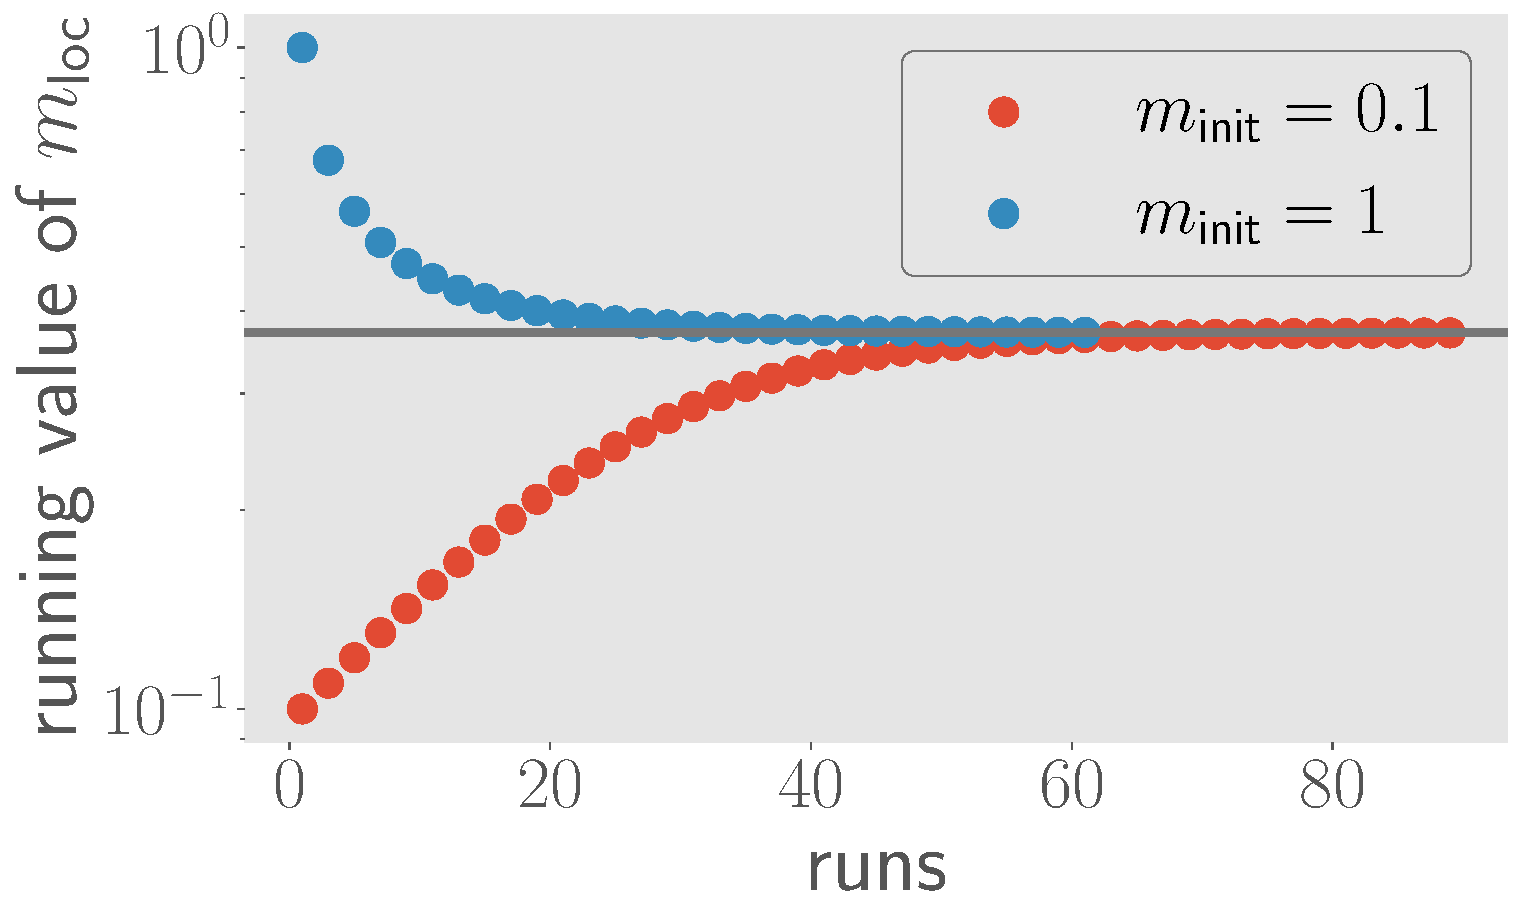
\includegraphics[width=0.8\textwidth]{ising_selfconsistency.pdf}
	\caption{Convergence of the local magnetisation to the self-consistent value after repeatedly solving the Hamiltonian and updating it with the solution.}
	\label{ising-selfconsistency}
\end{figure}

The more general approach to applying the mean field approximation can therefore be formalised as follows:
\begin{itemize}
	\item Figure out what the self-consistency equation is. It will be of the following generic form: y = f(y).
	\item Replace the fluctuations by an effective local mean field \(f(y)\), in order to obtain a simpler problem (the simplified Hamiltonian \(H_\text{MF}\)).
	\item Solve the simpler problem at a particular local site \(i\) by starting with some guess value of \(f(y)\), to calculate the mean field \(y^\prime\) from it.
	\item Create an updated Hamiltonian by setting \(y=y^\prime\).
	\item Solve this new Hamiltonian to obtain yet another updated \(y^\prime\), and keep repeating this until \(y\) does not change.
\end{itemize}

\end{document}
